\subsection{Anterior à modificação}

A região escolhida para o cenário 1 foi a interligação entre a subestação de Bouca e Zezere, na região central de Portugal como pode ser visto na Figura \ref{fig:caso1}. A mudança no cenário atual é a retirada de uma das duas linha que interligam o barramento da subestação de Bouca com o barramento de 145 kV de Zezere.

\vspace{3.3mm}

\begin{figure}[H]
	\centering
	\captionsetup{width=1\textwidth, font=footnotesize, textfont=bf}	
	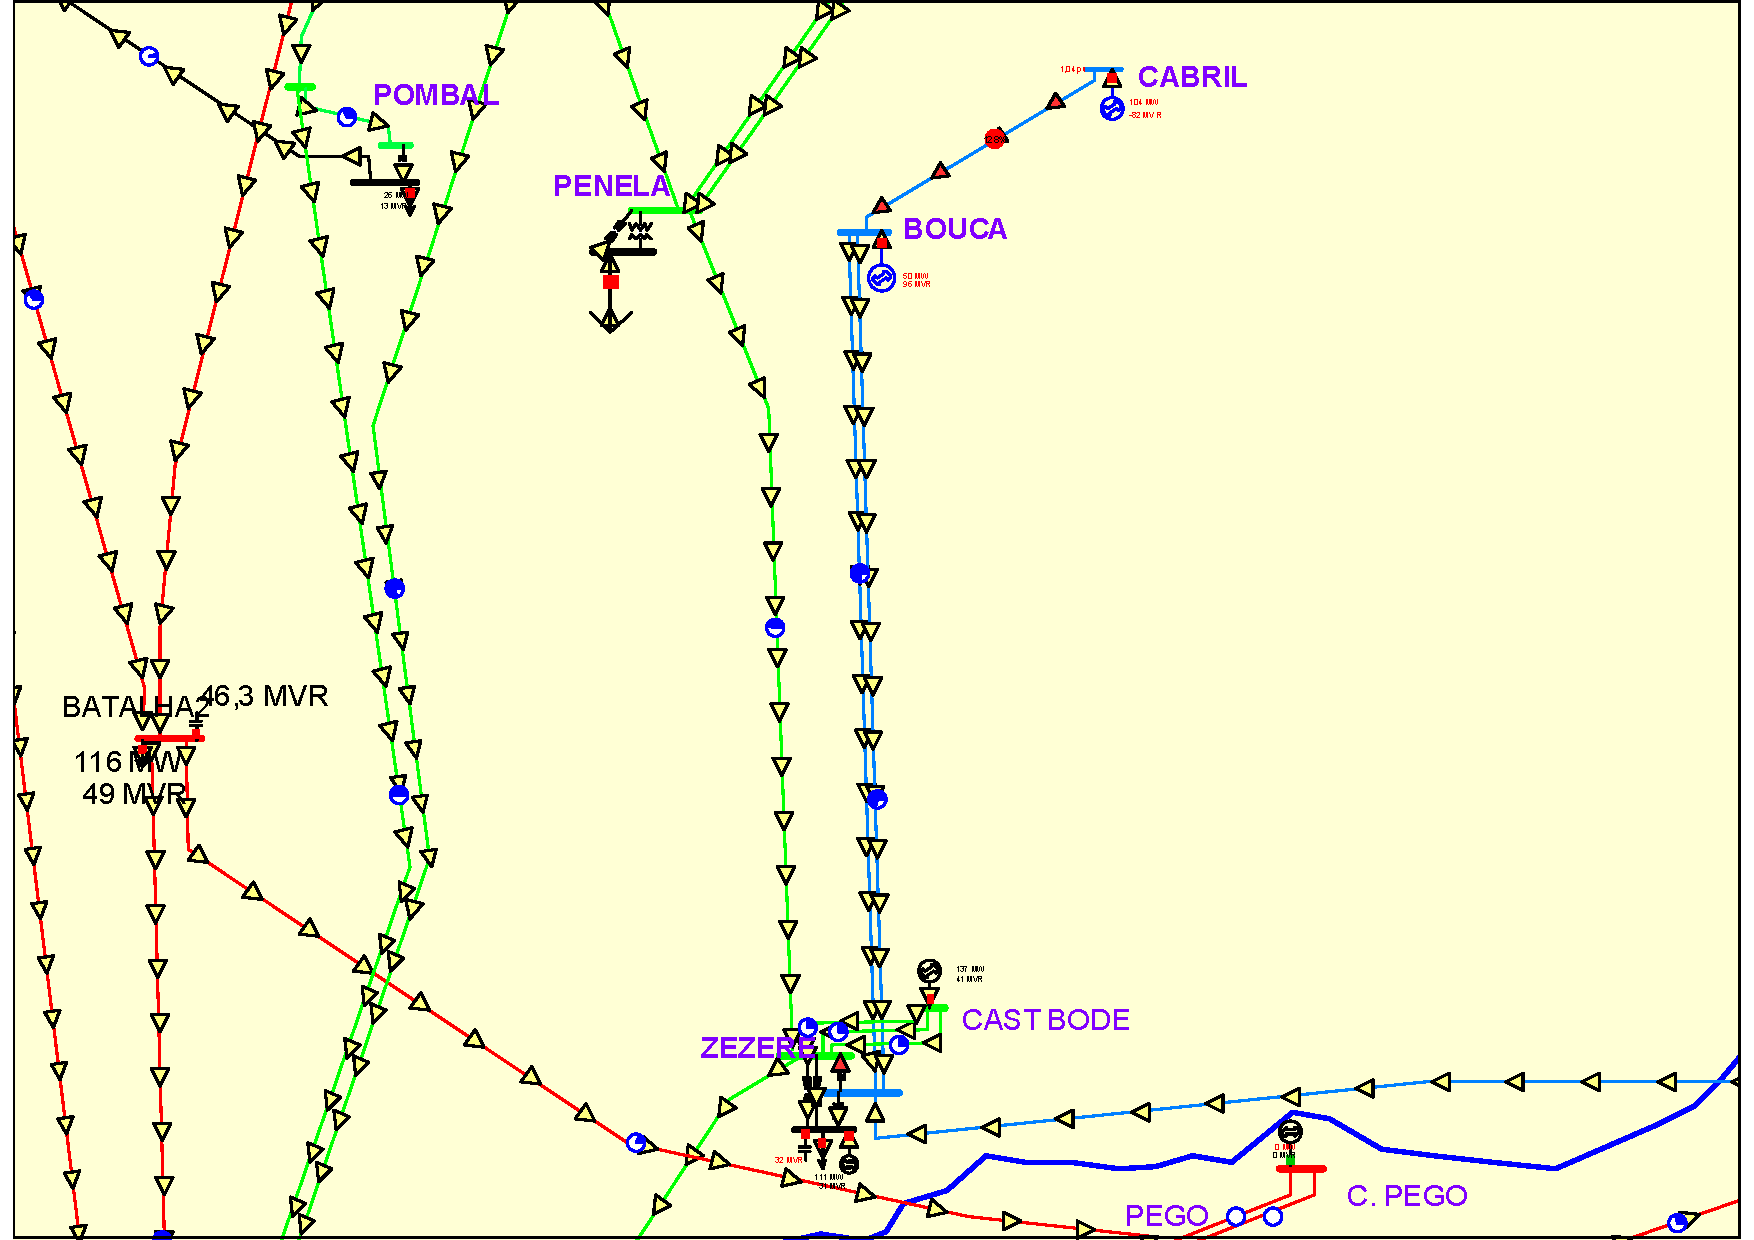
\includegraphics[width=1\linewidth]{img/caso1.pdf}
	\caption{Cenário 1, anterior à modificação}
	\vspace{-3.5mm}
	\caption*{Fonte: Caso Simulado no \textit{PowerWorld\textsuperscript{\textregistered} Simulator}}
	\label{fig:caso1}
\end{figure}

A subestação de Bouca se interliga apenas com o barramento de 145 kV de Zezere e com o barramento de Cabril, o qual possui uma unidade geradora de 104 MW. Existe apenas uma linha de Bouca a Zezere o qual apresenta uma sobrecarga 128\% no transito de potência no sentido Cabril Bouca. A interligação entre bouca e Zezere é feita por duas linhas que apresentam respectivamente  72,5\% e 72,6\% de carregamento.

A subestação de Zezere possui 3 barramentos; o primeiro de 145 kV que interligam a Bouca e Falaguei, o segundo que 230 kV que interligam Santarem, Penela e Cast Bode. O terceiro barramento de 63 kV é onde está conectado uma carga de 111M e um gerador de 22,1 MW. Os dados globais do sistema antes das alterações propostas estão dispostas na tabela \ref{tab:DadosGeraisIniciais}.

\begin{table}[H]
\centering
	\captionsetup{width=0.4\textwidth, font=footnotesize, textfont=bf}
    \begin{tabular}{|
  >{\columncolor[HTML]{333333}}l |c|c|l}
  \cline{1-3}
  {\color[HTML]{FFFFFF} }        & \cellcolor[HTML]{333333}{\color[HTML]{FFFFFF} MW} & \cellcolor[HTML]{333333}{\color[HTML]{FFFFFF} MVAr} &  \\ \cline{1-3}
  {\color[HTML]{FFFFFF} Perdas}  & 229,50                                            & -376,75  &  \\ \cline{1-3}
  {\color[HTML]{FFFFFF} Geração} & 6794,0                                             & -306,1  &  \\ \cline{1-3}
  {\color[HTML]{FFFFFF} Cargas}  & 6564,5                                            & 1814,2 &  \\ \cline{1-3}
  \end{tabular}
  \caption{Dados globais iniciais}
  \vspace{-3.5mm}
	\caption*{Fonte: Autoria Própria}
  \label{tab:DadosGeraisIniciais}
\end{table}

\begin{table}[H]
\centering
\captionsetup{width=0.4\textwidth, font=footnotesize, textfont=bf}
\begin{tabular}{lcc}
\multicolumn{3}{c}{\cellcolor[HTML]{333333}{\color[HTML]{FFFFFF} Carregamento das Linhas}} \\
\multicolumn{1}{c}{}          & \multicolumn{2}{c}{Carregamento (\%)}                \\
Cabril                              & \multicolumn{1}{l}{Bouca}            & 128,5         \\
Bouca                               & \multicolumn{1}{l}{Zezere}           & 73,4          \\
Falaguei                            & \multicolumn{1}{l}{Zezere}           & 52,6          \\
Panela                              & \multicolumn{1}{l}{Zezere}           & 47,1          \\
Zezere                              & \multicolumn{1}{l}{Santarem}         & 81,5          \\
Cast Bode                           & \multicolumn{1}{l}{Zezere}           & 25            \\
\multicolumn{3}{c}{\cellcolor[HTML]{333333}{\color[HTML]{FFFFFF} Tensão nas Barras}}       \\
\multicolumn{1}{c}{}           & Módulo                               & Ângulo        \\
Cabril                              & 1,04                                 & 30,889        \\
Bouca                               & 1,05                                 & 29,566        \\
Zezere                              & 1,0399                               & 22,006        \\
Falaguei                            & 1,03                                 & 30,919        \\
Panela                              & 1,0473                               & 26,098        \\
Santarem                            & 1,0269                               & 14,32         \\
Cast Bode                           & 1,04                                 & 22,019        \\
\multicolumn{3}{c}{\cellcolor[HTML]{333333}{\color[HTML]{FFFFFF} Geradores}}               \\
\multicolumn{1}{c}{}         & MW                                   & Mvar          \\
Cabril                              & 104,2                                & -82,29        \\
Bouca                               & 49,6                                 & 96,14         \\
Zezere                              & 22,1                                 & -23,24        \\
Cast Bode                           & 137,2                                & 41,46         \\
Falaguei                            & 148                                  & 65,76        
\end{tabular}
\caption{Dados Locais Iniciais}
  \vspace{-3.5mm}
	\caption*{Fonte: Autoria Própria}
  \label{tab:DadosLocaisIniciais}
\end{table}

% - sUBSECTION
\subsection{Análise do impacto da modificação}

\begin{figure}[H]
	\centering
	\captionsetup{width=1\textwidth, font=footnotesize, textfont=bf}	
	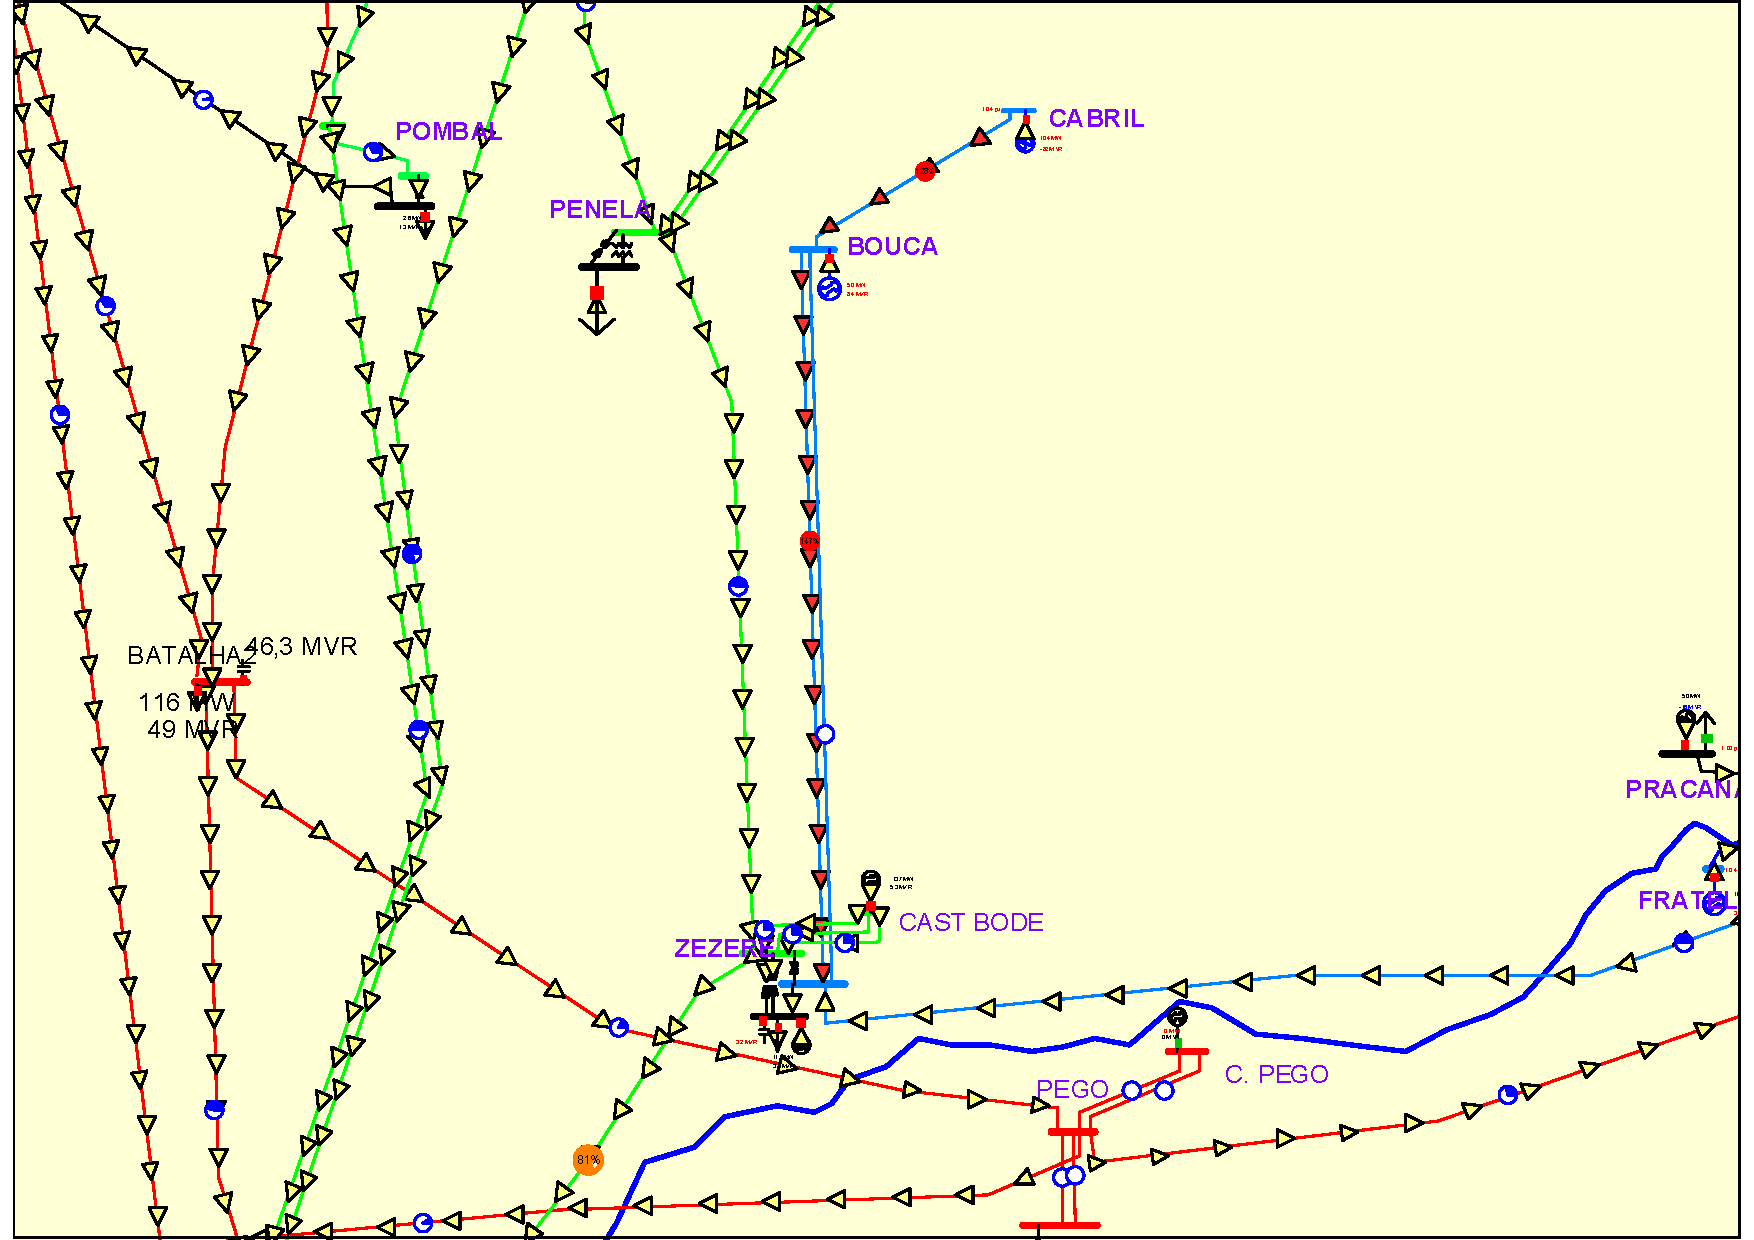
\includegraphics[width=1\linewidth]{img/caso1After.pdf}
	\caption{Satisfação do Consumo}
	\vspace{-3.5mm}
	\caption*{Fonte: Caso Simulado no \textit{PowerWorld\textsuperscript{\textregistered} Simulator}}
	\label{fig:caso1After}
\end{figure}

\subsubsection{Analisar geradores}

\begin{figure}[H]
	\centering
	\captionsetup{width=\textwidth, font=footnotesize, textfont=bf}	
	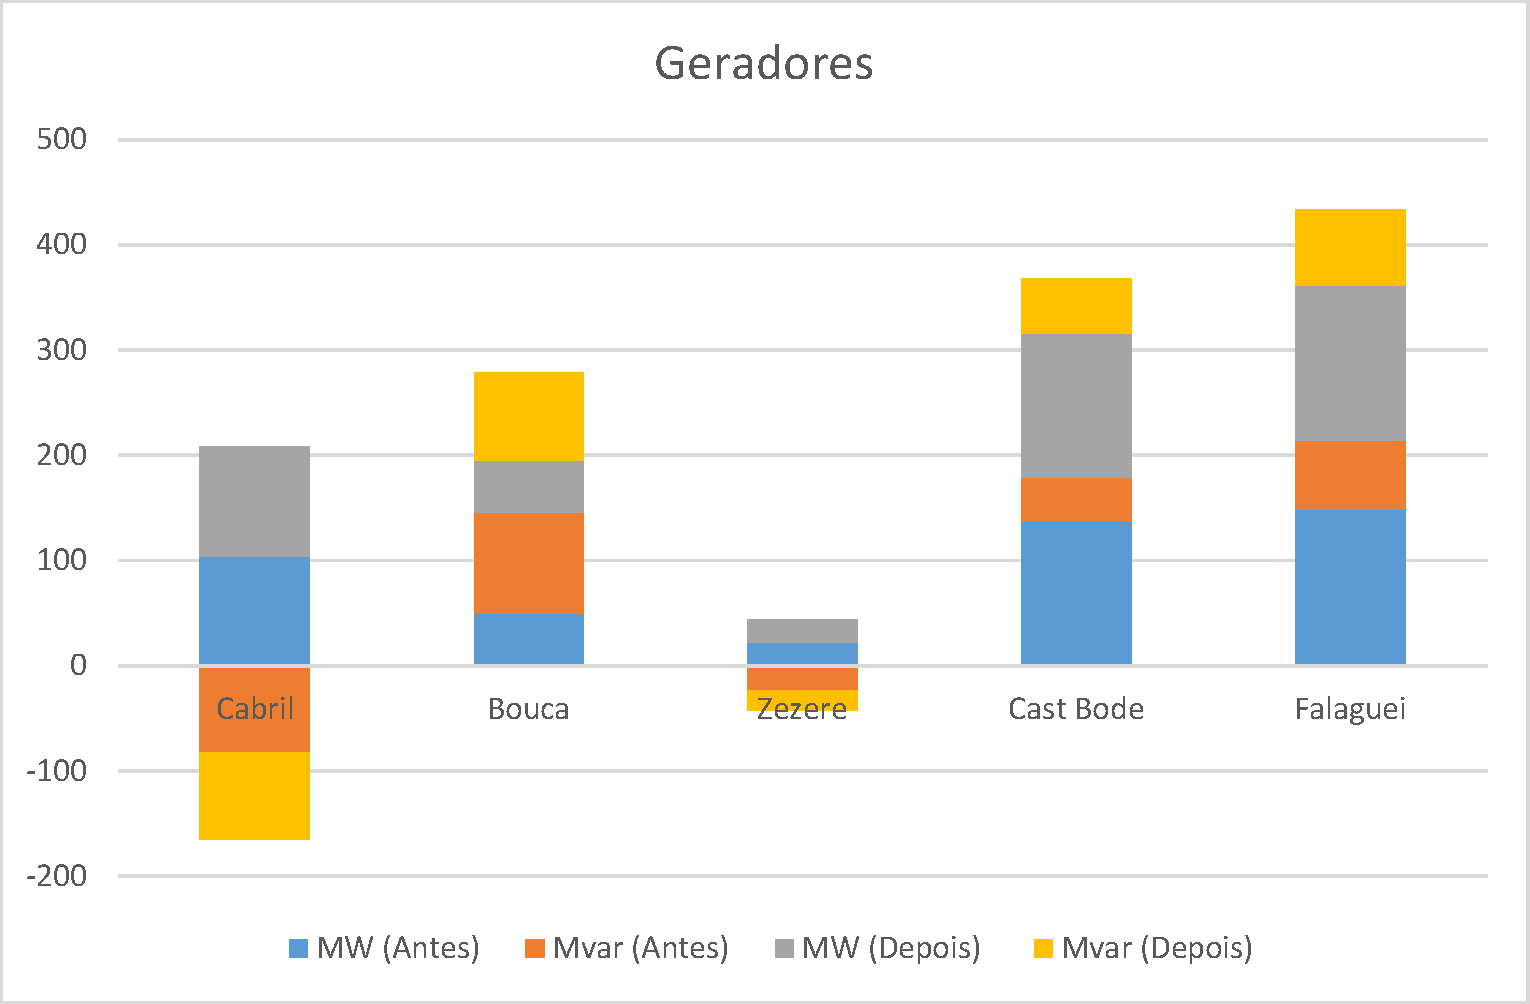
\includegraphics[width=\linewidth]{img/geradores_caso1.pdf}
	\caption{Análise dos geradores antes e após o cenário 1}
	\vspace{-3.5mm}
	\caption*{Fonte: autoria própria}
	\label{fig:geradores_caso1}
\end{figure}


\subsubsection{Análise das linhas}

\begin{figure}[H]
	\centering
	\captionsetup{width=\textwidth, font=footnotesize, textfont=bf}	
	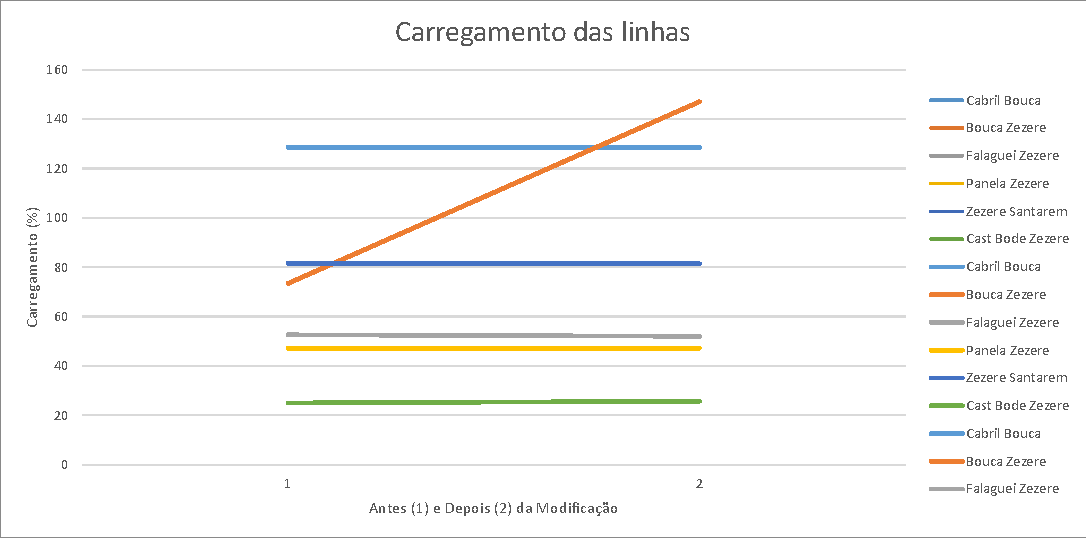
\includegraphics[width=0.9\linewidth]{img/carregamento_linhas_caso1.pdf}
	\caption{Análise do carregamento das linhas antes e após o cenário 1}
	\vspace{-3.5mm}
	\caption*{Fonte: autoria própria}
	\label{fig:carregamento_linhas_caso1}
\end{figure}

	% Mudança do trânsito de potência
	% Sobrecargas
    
\subsubsection{Análise dos barramentos}

\begin{figure}[H]
	\centering
	\captionsetup{width=\textwidth, font=footnotesize, textfont=bf}	
	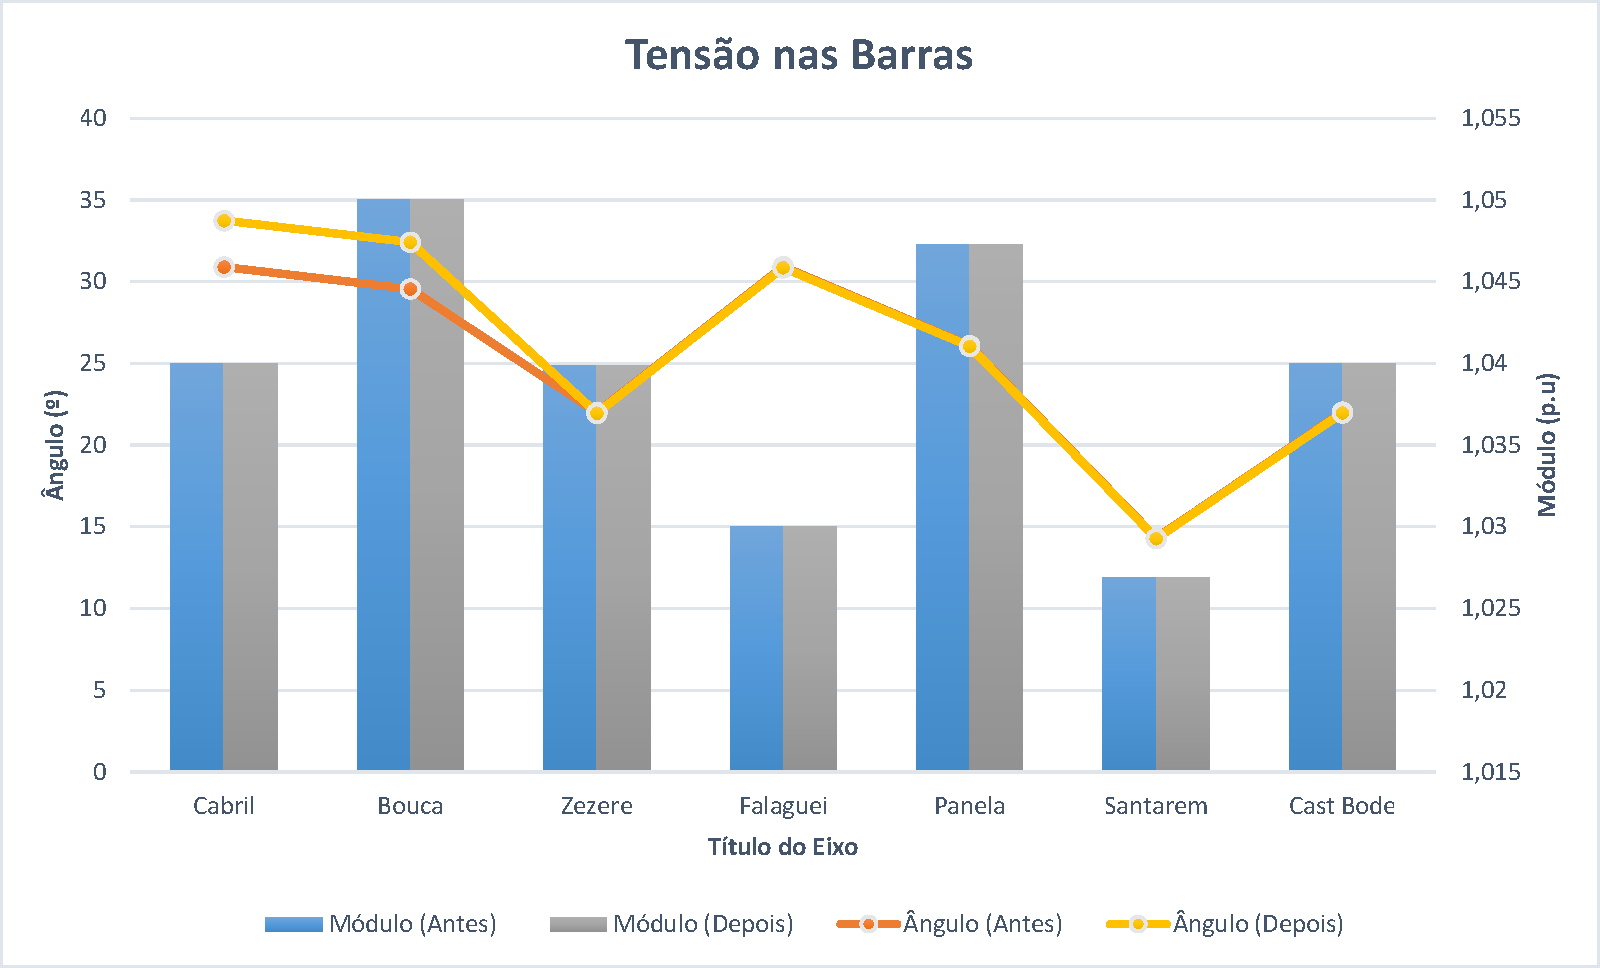
\includegraphics[width=\linewidth]{img/tensoes_barras_caso1.pdf}
	\caption{Análise dos Barramentos Antes e Após o Cenário 1}
	\vspace{-3.5mm}
	\caption*{Fonte: autoria própria}
	\label{fig:tensoes_barras_caso1}
\end{figure}
	% Tensões 
	% Ângulos